\documentclass[tikz]{standalone}
\usepackage{siunitx}
\usepackage{pgfplots}
\usepackage{graphicx}
\pgfplotsset{compat=newest}
\definecolor{photoncolor}{rgb}{0.65, 0.16, 0.16}
\begin{document}
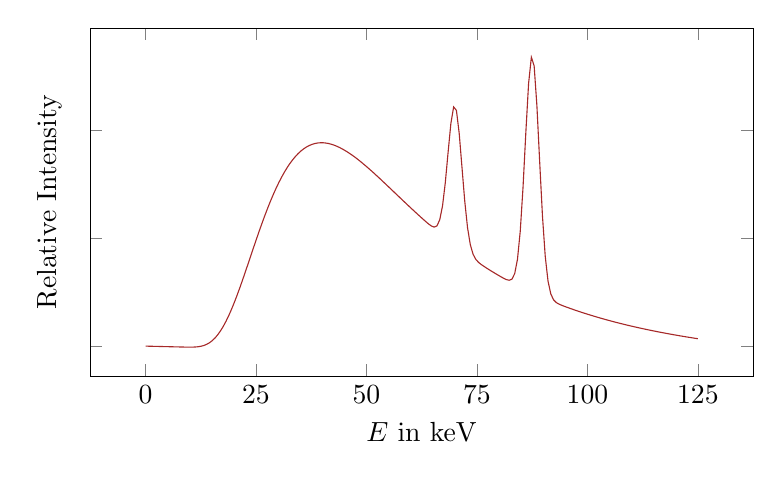
\begin{tikzpicture}
	\begin{axis}[
		xlabel={\( E \) in \si{\kilo\electronvolt}},
		ylabel={Relative Intensity},
		yticklabels={},
		xtick={0,1,2,3,4,5},
		xticklabels={\( 0 \),\( 25 \),\( 50 \),\( 75 \),\( 100 \),\( 125 \)},
		width=10cm,
		height=6cm,
	]
		\addplot [photoncolor,samples=200,mark=none,domain=0:5] {3000*e^(-8/x)*x^(-5)+1.3*e^(-((x-2.8)/0.09)^2)+2.2*e^(-((x-3.5)/0.09)^2) - x/40};
	\end{axis}
\end{tikzpicture}
\end{document}
